\documentclass[a4paper,12pt]{article}
\usepackage[T1]{fontenc}
\usepackage[utf8]{inputenc}
\usepackage{booktabs}
\usepackage{natbib}
\usepackage{amsmath}
\usepackage[colorlinks=true]{hyperref}
\usepackage[official]{eurosym}
\usepackage{graphicx}
\usepackage{rotating}
\usepackage{color}
\usepackage{fancyvrb}

\author{J. Ignacio Lucas Lledó}
\title{Notes on the fly project}
\begin{document}
\maketitle
\section{Delivery of oligonucleotides}
The oligonucleotides designed on \href{https://github.com/IgnasiLucas/fly/tree/master/results/2016-06-09}{2016-06-09} were ordered to biomers.net, and delivered. They are dry. Table~\ref{tab:oligos} specifies the yield and the corresponding amount of buffer required to dilute them to 100 pmol/$\mu$l.

\begin{table}
\begin{center}
\caption{Name and available amount (yield) of oligonucleotides received from biomers.net. `Volume' makes reference to the volume required to dissolve the corresponding oligonucleotides at 100 pmol/$\mu$l ($\mu$M).}\label{tab:oligos}
\vspace*{0.3cm}
\begin{tabular}{lrr|lrr}
\toprule
Name&Yield&Volume&Name&Yield&Volume\\
&(nmol)&($\mu$l)&&(nmol)&($\mu$l)\\
\midrule
Top1.1&82.6&826&Bot1.1&64.8&648\\
Top1.2&106.8&1068&Bot1.2&110.4&1104\\
Top1.3&94.9&949&Bot1.3&92.6&926\\
Top1.4&85.6&856&Bot1.4&75.8&758\\
Top2.1&78.9&789&Bot2.1&90.7&907\\
Top2.2&81.9&819&Bot2.2&97.4&974\\
Top2.3&100.5&1005&Bot2.3&84.2&842\\
Top2.4&88.4&884&Bot2.4&82.3&823\\
Top3.1&98.6&986&Bot3.1&87.1&871\\
Top3.2&95.2&952&Bot3.2&96.6&966\\
Top3.3&100.2&1002&Bot3.3&87.9&879\\
Top3.4&95.6&956&Bot3.4&78.7&787\\
A1.1&60.2&602&A2&65.9&659\\
A1.2&52.6&526&R1&78.7&787\\
A1.3&56.7&566&R2&60.0&600\\
A1.4&51.0&510&&&\\
\bottomrule
\end{tabular}
\end{center}
\end{table}

\section{DNA extraction test}
On September 13$^\mathrm{th}$ 2009, Dr. Carazo, Mrs. Sultanova, Mr. Andiç and I started the DNA extraction from 8 flies, following the \href{https://github.com/IgnasiLucas/fly/blob/master/doc/gbs.pdf}{GBS} protocol. Table~\ref{tab:flies} summarizes the procedure. Not that we needed 4 people to run this, but they all were interested in going through the protocol, which is great. The protocol is applied to each fly individually, with the aim of measuring how much DNA we can get from one fly. Four of the flies had their oviduct previously removed by Mrs. Sultanova. We want to make sure that the ovariectomy does not significantly reduce DNA yield.

\begin{table}
\begin{center}
\caption{Summary of the DNA extraction test.}\label{tab:flies}
\vspace*{0.3cm}
\begin{tabular}{cccll}
\toprule
Sample&Treatment&Elution ($\mu$l)&Conc.(ng/$\mu$l)&Yield (ng)\\
\midrule
1&--&100&4.240&424\\
2&--&100&0.978&98\\
3&--&100&3.600&360\\
4&--&100&1.790&179\\
5&ovariectomy&100&1.990&199\\
6&ovariectomy&100&3.980&398\\
7&ovariectomy&100&1.140&114\\
8&ovariectomy&100&1.530&153\\
\bottomrule
\end{tabular}
\end{center}
\end{table}

We ended up measuring DNA concentration 3 times, due to problems with the Qubit standards. The error `Incorrect standards' was apparently caused by the fact that the reagent had been kept in the fridge. I thought that it would be enough to wait for it to thaw, to bring it to room temperature. Plus, it is a very small amount of it that gets dissolved in the buffer, at room temperature. For whatever reason, the kit worked once we kept the reagent at room temperature. I thank Rebeca Dominguez, from the Evolutionary Genetics lab, her help to solve the problem.

The slight difference in average DNA concentration between control and ovariectomy samples is not significant, which is good news. I expect three samples, namely 1, 3, and 6, to have enough DNA left to run the rest of the protocol with them. I could add sample 5 to see what we get from it.

\section{Literature review}
Original motivation of classic life span QTL mapping studies was the elucidation of metabolic pathways involved in aging \citep{Nuzhdin2005}. I suspect that the biomedical interest in the mechanisms of aging preceded the interest in naturally occurring variation, as well as the real effect of the QTL identified in natural conditions. Several sex-specific life span QTL exist in autosomes of \emph{D. melanogaster} \citep{Nuzhdin1997,Pasyukova2000}. These QTL were originally identified using recombinant inbred lines (RIL) descended from two strains \citep{Nuzhdin1997}. In this design, the dominance of the QTL is not known, since only homozygous genotypes are produced \citep[][page 432]{Lynch1998}. However, the quantitative complementation test with deficencies used to refine the QTL \citep{Pasyukova2000} seems to assume that one of the alleles is at least partially recessive.

\citet{Crow2008} mentions the genetic basis of heterosis as one of the main mid-century controversies in population genetics. He is very clear that the debate between dominance and overdominance was resolved in favor of the dominance hypothesis. That is, both the inbreeding depression and the hybrid vigor (heterosis) are mostly due to recessive deleterious alleles that become either expressed upon inbreeding or concealed upon hybridization. A review \citep{Charlesworth2009} cites another work by James F. Crow that I cannot access (volume 9 of the Oxford Series in Evolutionary Biology), in which the author shows evidence of 30\% of autosomes isolated from natural populations of \emph{D. melanogaster} being lethal in homozygosis. The same cannot be true for sex chromosomes, of course. Among the 70\% of natural chromosomes that are not recessive lethals, homozygosity reduces survival to adulthood in 84\%.

Full-sib mating during 10 generations is expected to produce an inbreeding coefficient of 0.886. This is the probability at any locus that the two copies inherited from the parents are identical by descent; that is, they are exact copies of the same chromosome in one of the recent ancestors. But how is this identity-by-descent distributed along a chromosome? It is not random, but clustered, because of linkage. We expect an alternative sequence of fragments that are either identical by descent or not. That is, the inbreeding itself already produces a mosaic of heterozygosity and homozygosity. The question is how long the pieces are. Too short IBD tracts would require very dense markers. According to \citet{Franklin1977}, previous authors (Bennet and Fisher) had supposed that `after a long number of generations of inbreeding the number of heterogenic segments will be approximately distributed as a Poisson variable, and that the distribution of the length of each segment ($x$) will tend to a negative exponential $(1/a)e^{-x/a}$.' However, this assumptions are not satisfactory, especially for the first few generations of inbreeding. Taking into account that there is no crossing-over in \emph{Drosophila males}, the probability that two loci in the same chromosome are homozygous by descent after one generation of sib mating is $(1/32)(3 + 3\lambda_f + \lambda^2_f + \lambda^3_f)$ \citep{Franklin1977}, where $\lambda_f$ is the linkage parameter $1-2y_f$, representing the probability of recombination in the female.

The suggestion given by Dr. Carazo of using simulations is actually good. I started learning to use simuPOP.

\section{Enzymatic digestion of DNA samples 1, 3, 5, and 6}
I run the digestions as described on table~\ref{tau:digestion}, for above 4 hours, at 37$^\circ$C. Together with Muhammed Andiç, we also cleaned up the reaction with magnetic beads. We used a 1:1 ratio of beads to DNA, and eluted with water (40 $\mu$l). 

\begin{table}
\begin{center}
\caption{Digestion reactions.}\label{tau:digestion}
\vspace*{0.3cm}
\begin{tabular}{cccccc}
\toprule
      &DNA&H$_2$O&10$\times$ buffer&NspI&Total\\
Sample&($\mu$l)&($\mu$l)&($\mu$l)&($\mu$l)&($\mu$l)\\
\midrule
1&80&207&32&1&320\\
3&80&207&32&1&320\\
5&80&207&32&1&320\\
6&80&207&32&1&320\\
\bottomrule
\end{tabular}
\end{center}
\end{table}

\section{Literature review}
From page 489 of \citet{White1973}: "The adaptive significance of achiasmatic meiosis is not entirely clear. Obviously it has been evolved repeatedly in at least ten major groups of animals. In those cases where achiasmatic meiosis is confined to one sex, we have far too little information as to the chiasma frequency in the other sex. If it were generally true that in the `chiasmatic sex' there is only one chiasma per bivalent, we might assume that selection for a low level of genetic recombination \emph{per se} had led to total loss of chiasmata in one sex. If, on the other hand, absence of chiasmata in one sex is generally accompanied by a fairly high chiasma frequency in the other, this explanation obviously would not hold. Only evidence from species that had acquired achiasmatic mechanisms fairly recently in their phylogeny would be significcant from this point of view (\emph{Tipula caesia} would be relevant -- \emph{Drosophila} spp. would not). The only evidence on this point seems to be the grasshopper \emph{Thericles whitei}, with no chiasmata in the male and a very low chiasma frequency in the female; it obviously supports the hypothesis of selection for low levels of recombination."

However, selection for low levels of recombination would not explain why the achiasmatic sex is nearly always the heterogametic sex \citep{Burt1991}. \citet{White1973} also mentions the hypothesis of achiamatic spermatogenesis being an adaptation to tolerate inversion-heterozygosity. However, no evidence supports this hypothesis.

More recently, \citet{Lenormand2016} mention two more hypotheses: first, that achiasmy may have evolved as a side effect of selection to suppress recombination between the sex chromosomes \cite{Haldane1922,Huxley1928}. And second, that it evolved as a way to promote tight linkage without suppressing recombination on the X or Z chromosome \citep{Lenormand2005}.

Well, I cannot review now all the hypotheses now. If anything, I should relate the results of the simulations to the theoretical expectations of the variance in inbreeding coefficient \citep{Cockerham1968,Franklin1977}. It seems that multiple linked loci in sex chromosomes have received relatively little attention in the literature \citep{Bennett1963,Owen1988}.

\section{Annealing of adapters}
On September 28th, Muhammed and I prepared 100 ml of 1$\times$ TE buffer, following a recipe online: 1.0 ml 1M Tris pH 8.0, 0.2 ml EDTA 0.5M, and 98.8 ml H$_2$O. We also prepared annealing buffer, according to the protocol, and suspended all the oligonucleotides in TE buffer to 100 $\mu$M, according to the volume specified on table~\ref{tab:oligos}. Finally, we prepared 10 $\mu$l of annealed adapters of each type.

\section{Quantification with Agilent Bioanalyser}
Amparo Martínez, from the Sequencing Service, sent the results from the Bioanalyser run. The four samples have a very similar profile (Figure~\ref{fig:digestion}), which looks like the result of a successful digestion followed by a more aggressive selection of long fragments that I expected from a 1:1 ratio of magnetic beads to DNA. Next time, I should use a more generous proportion of beads. Table~\ref{tau:fragments} shows some additional details. I note that the amount of DNA available is now an order of magnitude lower than what I had for the \emph{Coregonus} samples.

\begin{figure}
\centering{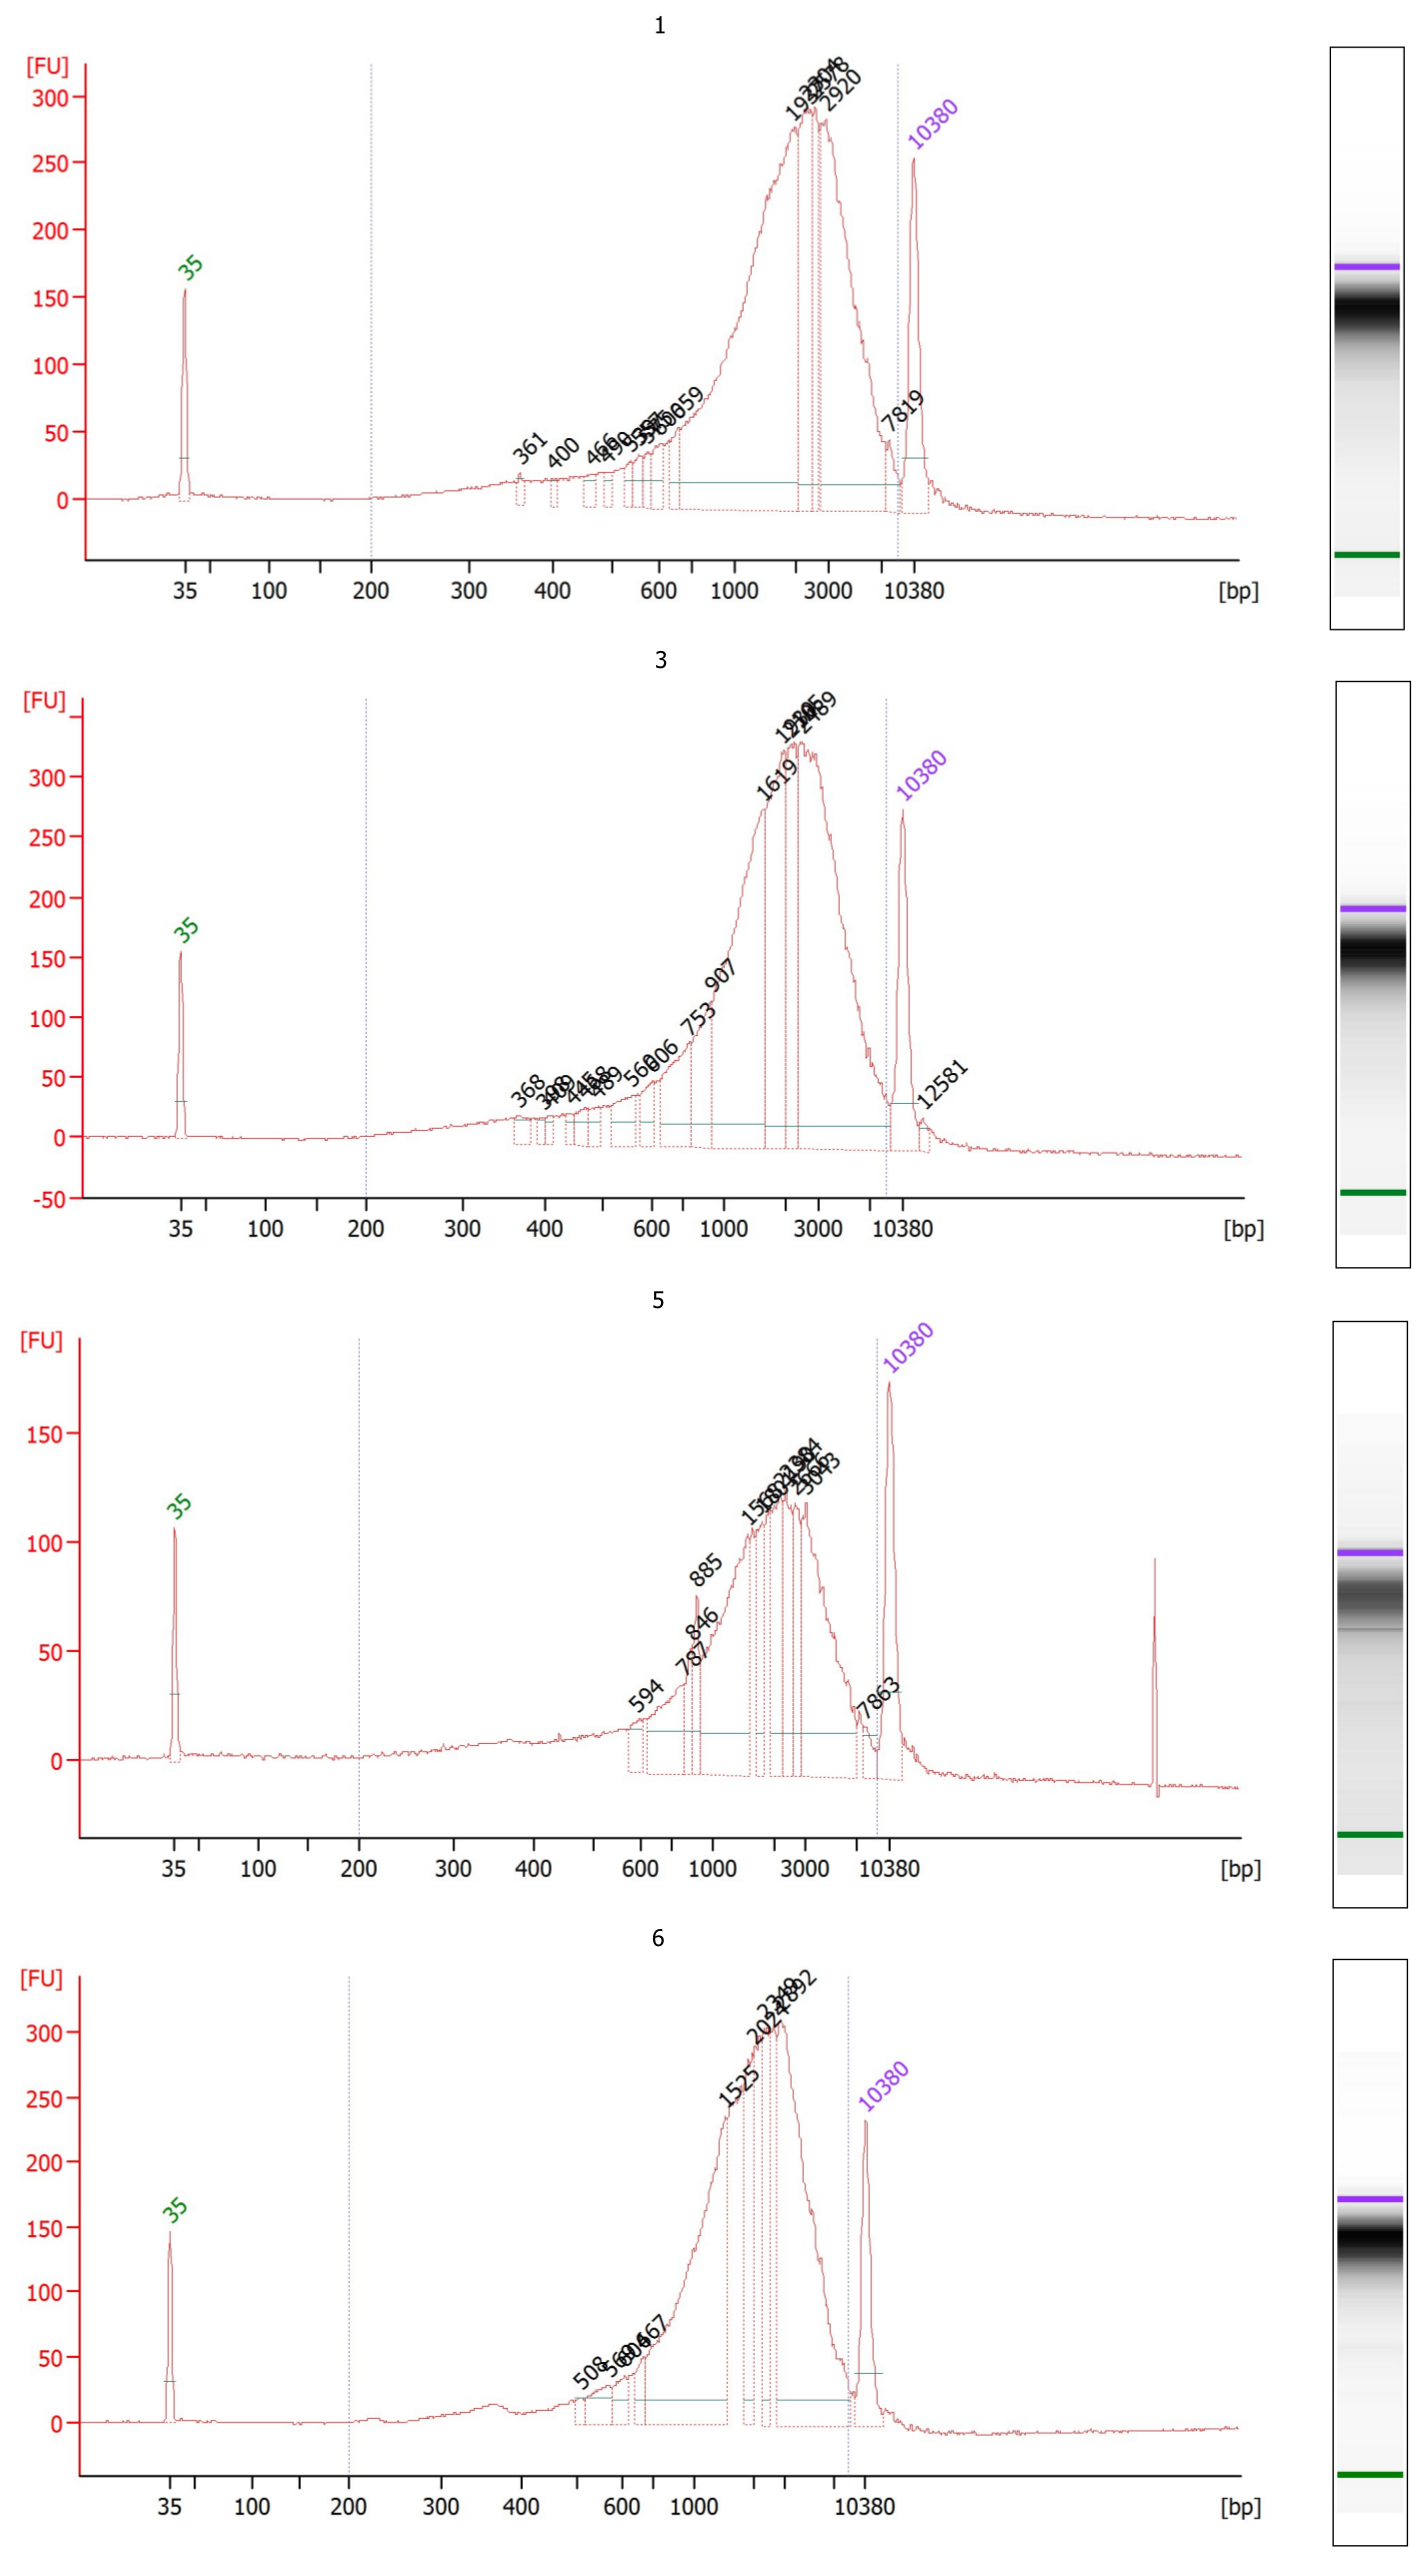
\includegraphics[width=11cm]{images/Digestion.png}}
\caption{Electropherograms from the high-sensitivity DNA assay of the four samples.}\label{fig:digestion}
\end{figure}

\begin{table}
\begin{center}
\caption{Distribution of DNA fragments between 40 and 9000 bp. `Size' refers to the average fragment size. For total mass of DNA left over, a volume of 35 $\mu$l is assumed to be left. The average fragment mass (Frag.Mass) is calculated in two ways. First, by dividing the overall concentration by the overall molarity (Frag.Mass.1); and then, by applying the formula for the molecular mass of double stranded DNA to the average length of the fragments (i.e., $607.4x+157.9$ g/mol; Frag.Mass.2).}\label{tau:fragments}
\vspace*{0.3cm}
\begin{tabular}{lrrrrrr}
\toprule
&Size&Conc.&Molarity&Left over&Frag.Mass.1&Frag.Mass.2\\
Sample&(bp)&(pg/$\mu$l)&(pmol/l)&(ng)&(ng/fmol)&(ng/fmol)\\
\midrule
1&2206&1425.92&3042.0&49.91&0.468744&1.34008\\
3&2239&1439.86&2484.9&50.40&0.579444&1.36013\\
5&2022&1113.97&3509.8&38.99&0.317388&1.22832\\
6&2376&1523.30&2066.7&53.32&0.737069&1.44334\\
\bottomrule
\end{tabular}
\end{center}
\end{table}

\section{Ligation of adapters}
In folder 2016-10-04, I calculate the composition of the ligation reactions to have a 10-fold excess of adapters to DNA fragment ends. On table~\ref{tau:working} I show the composition and final concentrations of the working solutions of the four adapters, required to prepare the ligation reactions specified on table~\ref{tau:ligation}. Importantly, I decide to assign adapters 1.1, 1.2, 1.3, and 1.4 to samples 1, 3, 5, and 6, respectively. See table~\ref{tau:codewords}. 

\begin{table}
\begin{center}
\caption{Composition and final concentration of the working solutions of adapters for the ligation reactionson table~\ref{tau:ligation}. The buffer must be 1$\times$ annealing buffer. Amounts are $\mu$l, except the final molarity, in the last column, in pmol/$\mu$l.}\label{tau:working}
\vspace*{0.2cm}
\begin{tabular}{cccccc}
\toprule
Sample&Adapter&1$\times$ buffer&15 $\mu$M Stock&Total&pmol/$\mu$l\\
\midrule
1&1.1&8.580&1.420&10.00&2.13\\
3&1.2&8.840&1.160&10.00&1.74\\
5&1.3&8.362&1.638&10.00&2.46\\
6&1.4&9.036&0.964&10.00&1.45\\
\bottomrule
\end{tabular}
\end{center}
\end{table}

\begin{table}
\caption{Volumes of reactants in the ligation reactions. All in $\mu$l. T4 ligase is at 2000000 U/ml.}\label{tau:ligation}
\vspace*{0.2cm}
\begin{tabular}{cccccccc}
\toprule
Sample&DNA&10$\times$ Buffer&Adapter&1.5 M NaCl&T4&H$_2$O&Total\\
\midrule
1&35&4.40&1.00&1.10&2.00&0.50&44.00\\
3&35&4.40&1.00&1.10&2.00&0.50&44.00\\
5&35&4.40&1.00&1.10&2.00&0.50&44.00\\
6&35&4.40&1.00&1.10&2.00&0.50&44.00\\
\bottomrule
\end{tabular}
\end{table}

\begin{table}
\begin{center}
\caption{Adapters and codewords assigned to the DNA samples.}\label{tau:codewords}
\vspace*{0.2cm}
\begin{tabular}{ccl}
\toprule
Sample&Adapter&Codeword\\
\midrule
1&1.1&TTGATCCAGT\\
3&1.2&GATCAGGCAGT\\
5&1.3&CCAGCTTGT\\
6&1.4&AGCTGAAT\\
\bottomrule
\end{tabular}
\end{center}
\end{table}

Just to have a graphic representation of the adapters and the expected DNA fragments, this is how they should look like after ligation (adapter 1.1 represented):
\fvset{fontsize=\scriptsize,commandchars=\\\{\}}
\begin{flushleft}
\begin{tabular}{l}
   \Verb+ ACACTCTTTCCCTACACGACGCTCTTCCGA\textcolor{red}{TTGATCCAGT}CATG\textcolor{blue}{YNNNNNNNNNNNRCATG}\textcolor{red}{ACTGGATCAA}TCGGAAGAGCACACGTCTGAACTCCAGTCAC+\\[-4pt]
   \Verb+   |||      |        |||||||||||||||||||||||||||||||||||||||||||||||||||||||||||||        |      |||+\\[-10pt]
   \begin{turn}{180}
      \Verb+ACACTCTTTCCCTACACGACGCTCTTCCGA\textcolor{red}{TTGATCCAGT}CATG\textcolor{blue}{YNNNNNNNNNNNRCATG}\textcolor{red}{ACTGGATCAA}TCGGAAGAGCACACGTCTGAACTCCAGTCAC+
   \end{turn}
\\
\end{tabular}
\end{flushleft}

The codeword is in red, and the genomic fragment in blue. Note that the restriction site, RCATGY, is not present in the ligation product (R is G or A, and Y is C or T). This allows me to digest a second time, and get rid of chimeric fragments.

On October 5$^\mathrm{th}$, I prepared the working solution of the annealed adapters, and the following day I set up the ligation reaction. I then realized the available T4 DNA ligase was at 400000 U/ml, instead of 2000000 U/ml. I decided to double the amount of T4 ligase, and adjust the amount of buffer. I also noticed that sample 6 did not have more than 30 $\mu$l of DNA. Thus, I changed the composition of the reaction accordingly. However, I note that I used 1 $\mu$l of adapters at a slightly higher concentration than necessary to achive the 10-fold excess, because the working solution of adapters was already prepared, and I didn't want to re-calculate the whole thing. See table~\ref{tau:ligation2} for the current composition of the ligation reaction.

\begin{table}
\caption{Current composition of the ligation reaction, after necessary adjustments. All amounts are in $\mu$l. T4 ligase was actually at 400000 U/ml.}\label{tau:ligation2}
\vspace*{0.2cm}
\begin{tabular}{cccccccc}
\toprule
Sample&DNA&10$\times$ Buffer&Adapter&1.5 M NaCl&T4&H$_2$O&Total\\
\midrule
1&35&4.62&1.00&1.10&4.00&0.50&46.22\\
3&35&4.62&1.00&1.10&4.00&0.50&46.22\\
5&35&4.62&1.00&1.10&4.00&0.50&46.22\\
6&30&4.02&1.00&1.10&4.00&0.25&40.37\\
\bottomrule
\end{tabular}
\end{table}

\section{Second digestion}
The second digestion is meant to break chimeric fragments. The adapters will not be cleaved because they were designed not to reproduce the cut site. I do not want to clean up the ligation reaction. In the worse case, I will not get rid of the chimeras. But I don't want to loose DNA. So, I count the total ligation volumes (table~\ref{tau:ligation2}) as DNA volumes in the second digestion reactions specified on table~\ref{tau:digestion2}.

\begin{table}
\begin{center}
\caption{Second digestion reactions.}\label{tau:digestion2}
\vspace*{0.3cm}
\begin{tabular}{cccccc}
\toprule
      &DNA&H$_2$O&10$\times$ buffer&NspI&Total\\
Sample&($\mu$l)&($\mu$l)&($\mu$l)&($\mu$l)&($\mu$l)\\
\midrule
1&46.22&119.17&18.49&1&184.88\\
3&46.22&119.17&18.49&1&184.88\\
5&46.22&119.17&18.49&1&184.88\\
6&40.37&103.96&16.15&1&161.48\\
\bottomrule
\end{tabular}
\end{center}
\end{table}

\section{Size selection}
I plotted the expected shape of the electropherogram, using data from the in silico digestion with the pattern RCATGY (2016-04-12). The result, shown in figure~\ref{fig:expected}, is remarkably similar to the observed electropherograms after digestion (figure~\ref{fig:digestion}).

\begin{figure}
\centering{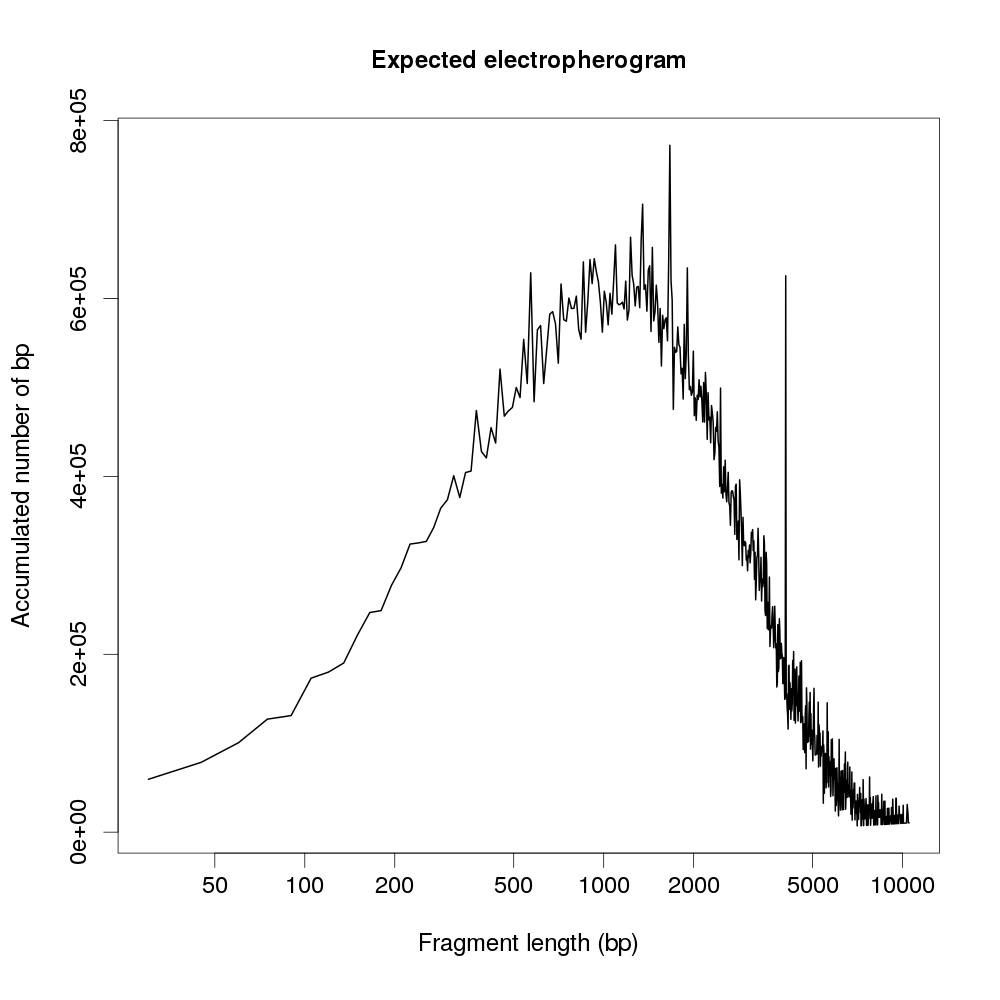
\includegraphics[width=11cm]{../results/2016-04-12/electropherogram.png}}
\caption{Expected shape of the electropherogram of digested DNA.}\label{fig:expected}
\end{figure}

In any case, from those figures it is not immediate to know the number of loci in a size range. The use of magnetic beads for size selection is tricky, because very precise volumes need to be measured, some DNA is lost, and the range is wider and less reproducible than if selected with a Blue Pippin. So, wide size ranges are convenient in this case. Therefore, I should move the range in the direction of lower number of fragments, so that a tighter control in the number of fragments is possible. After looking at the ratios of beads to DNA required for each range, I realize I cannot aim at fragments just between 500 and 800 bp, but rather between 450 and 1000 bp. Because I will use 300 bp, paired end reads, I stick to this range. Finally, I use beads to sample ratios of 0.600 (right-side selection at $\sim900$ bp) and 0.645 (left-side selection at $\sim350$ bp. I expect less than 33000 loci, according to results from the 2016-04-12/RCATGY folder. Given that the total volumes are either 184.88 or 161.48 $\mu$l, this translates into the volumes specified on table~\ref{tau:sizeselection}. I elute with 10 $\mu$l.

I have two different batches of magnetic beads. One is a free, 5-ml sample of NucleoMag\textsuperscript{\textregistered} NGS Clean-up and Size Select (Machery-Nagel), sent by Purificación Carrasco (Cultek S.L.U.) on July 1st 2016. A 50 ml bottle was offered then for \euro{}689.11 (VAT included). The other is a smaller sample of the CleanPCR product by CleanNA, sent on September 21st 2016 by Carmen Llorca (Labclinics S.A.). The 50 ml bottle of CleanPCR is offered for \euro{}475.20 + 21.0\% VAT $=$ \euro{}574.99.

I used CleanPCR with sample 1, and NucleoMag with samples 3, 5, and 6, for comparison. It is possible that the two batches produce different fragment size ranges \citep{Meyer2010}.

\begin{table}
\begin{center}
\caption{Volumes of DNA sample, bead suspension and ethanol to be added during right-side selection (Beads 1, 0.600:1 ratio), left-side selection (Beads 2; 0.645:1 ratio), and washing steps (ethanol). All in $\mu$l.}\label{tau:sizeselection}
\vspace*{0.3cm}
\begin{tabular}{ccccc}
\toprule
Samples&DNA&Beads 1&Beads 2&Ethanol\\
\midrule
1, 3, 5&184.88&110.93&8.32&$2\times 305.00$\\
6&161.48&96.89&7.27&$2\times 305.00$\\
\bottomrule
\end{tabular}
\end{center}
\end{table} 

\section{Amplification PCR. October 25, 2016}
After size selection I do not expect to have more than 2 ng of DNA per sample. I will not quantify before amplification, in order to save DNA and because I would not trust so small measures.

I realized I did not have the Phusion\textsuperscript{\textregistered} High-Fidelity PCR Master Mix with HF Buffer, but simply the Phusion High-Fidelity PCR Kit. Thus, the PCR reaction was like in table~\ref{tau:PCR}. I regreted the mistake, because I suspect pipetting accuracy was far from perfect with new tips that I don't trust. In addition, I note that by mistake I used a primer concentration of 0.2 $\mu$M, instead of the recommended 0.5 $\mu$M.

When reading the manual of Phusion High-Fidelity PCR Kit, I noticed the recommendation of running a 2-steps PCR with primers $>20$ nucleotides and with $T_m \ge 69^\circ$C. While the melting temperatures of the portions of the primers that anneal during the first and second cycle don't seem to be larger than 69$^\circ$C (table~\ref{tau:primers}), actually when using the ThermoFisher $T_m$ calculator, they are. Thus, a 2-step PCR programme is recommended, with a unique temperature of 72$^\circ$C for both annealing and extension. I finally gave only 20 s for these steps, which in retrospect seem too short (table~\ref{tau:pcrprogramme}).

After setting up the PCR reaction, I received Sibelle's Vilaça suggestion. She cites \citet{Meyer2010}, a protocol using the same PCR kit that I use, and in a similar application. They recommend the exact same reaction that I set up (table~\ref{tau:PCR}), including the 0.2 $\mu$M primers. However, the programme they suggest is different from mine (see table~\ref{tau:pcrprogramme}). It is unclear if the difference is justified by the use of slightly shorter primers, or if they just overrode \citet{Meyer2010} recommendation for some reason.

Because we have 4 differently indexed first primers, I prepared four primer mixtures (table~\ref{tau:index}). During preparation, I commited the mistake of adding 1 $\mu$l of 100 $\mu$M primer A1.1 directly to the template DNA of sample 1, instead of adding it to the corresponding primer mix. Because that would be a too high primer concentration, I decided to clean up sample 1's DNA with magnetic beads again, using a 0.7 beads to DNA ratio. Again, I used the CleanPCR brand, although the comparison with the other brand may be affected by this additional step.

\begin{table}
\begin{center}
\caption{PCR reactions in 50 $\mu$l. 10 $\mu$l of 10 $\mu$M Primer Mix may be prepared with 1 $\mu$l 100 $\mu$M Primer 1 $+$ 1 $\mu$l 100 $\mu$M Primer 2 $+$ 8 $\mu$l nuclease-free water.}\label{tau:PCR}
\vspace*{0.2cm}
\begin{tabular}{lrr}
\toprule
Component&Volume ($\mu$l)&Final conc.\\
\midrule
H$_2$O&27.5&\\
5$\times$ HF buffer&10.0&1$\times$\\
10 mM dNTPs&1.0&200 $\mu$M each\\
10 $\mu$M Primer Mix&1.0&0.2 $\mu$M\\
Template DNA&10.0&\\
Phusion DNA Pol.&0.5&0.02 U/$\mu$l\\
\midrule
Total&50.0&\\
\bottomrule
\end{tabular}
\end{center}
\end{table}

\begin{table}
\begin{center}
\caption{Amplification primers. These properties were calculated with an online \href{http://biotools.nubic.northwestern.edu/OligoCalc.html}{oligonucleotide properties calculator} \cite{Kibbe2007}. Different properties are obtained with the ThermoFisher \href{https://www.thermofisher.com/es/es/home/brands/thermo-scientific/molecular-biology/molecular-biology-learning-center/molecular-biology-resource-library/thermo-scientific-web-tools/tm-calculator.html}{Tm calculator}.}\label{tau:primers}
\vspace*{0.2cm}
\begin{tabular}{lccccc}
\toprule
&Primer 1a&Primer 1b&Primer 1c&Primer 1d&Primer 2\\
\midrule
Length (bp)&63&63&63&63&55\\
Molecular weight (g/mol)&19511.7&19545.7&19536.7&19536.7&16719.9\\
Basic T$_M$ First cycle ($^{\circ}$C)&65.7&65.7&65.7&65.7&64.4\\
52 mM Na$^{+}$ T$_M$ 1$^{st}$ cycle ($^{\circ}$C)&75.0&75.0&75.0&75.0&73.3\\
Basic T$_M$ Later cycles ($^{\circ}$C)&75.7&76.4&76.4&76.4&74.3\\
52 mM Na$^{+}$ T$_M$ Later ($^{\circ}$C)&87.2&88.0&88.0&88.0&85.7\\
\bottomrule
\end{tabular}
\end{center}
\end{table}

\begin{table}
 \begin{center}
  \caption{PCR programme. In parenthesis, values recommended by \citet{Meyer2010}, if different from the ones used.}\label{tau:pcrprogramme}
  \vspace*{0.3cm}
  \begin{tabular}{lccl}
   \toprule
Step&Temp.($^\circ$C)&Time (s)&\\
   \midrule
Initial denaturation&98&30&\\
Denaturation&98&\multicolumn{1}{c|}{10}&\\
Annealing&72 (60)&\multicolumn{1}{c|}{10 (20)}&12$\times$\\
Extension&72&\multicolumn{1}{c|}{10 (20)}&\\
Final extension&72&600&\\
Hold&4&$\infty$&\\
   \bottomrule
  \end{tabular}
 \end{center}
\end{table}

\begin{table}
 \begin{center}
  \caption{Indexing of samples.}\label{tau:index}
  \begin{tabular}{cccc}
   \toprule
Sample&Primer 1&Primer 2&Index\\
   \midrule
1&A1.1&A2&CTTGAGTC\\
3&A1.2&A2&GAACGCTG\\
5&A1.3&A2&GCCAGGTT\\
6&A1.4&A2&GCGTTAGC\\
   \bottomrule
  \end{tabular}
 \end{center}
\end{table}

\section{Clean-up and Bioanalyser quantification. October 26, 2016.}
I cleaned up the PCR reactions using a 0.8:1 beads to DNA ratio. Again, sample 1 was treated with the CleanPCR suspension, and the others with Machery Nagel's NucleoMag. I eluted with 10 $\mu$l of water. Then, I took the samples to the Sequencing Services to be quantified with the High Sensitivity Bioanalyser chip.

On October 27\textsuperscript{th}, A. Martínez sent me the electropherograms, shown on figure~\ref{fig:sizeselection}. The figure confirms that the ligation of adapters, the size selection, and the PCR worked more or less as expected. The only disappointment is that the Machery Nagel magnetic beads have quite different affinity for DNA than expected, which resulted in a shift of the selected size range towards larger fragments in samples 3, 5, and 6. I therefore, need to repeat the size selection on those samples, using the CleanPCR product.

\begin{figure}
\centering{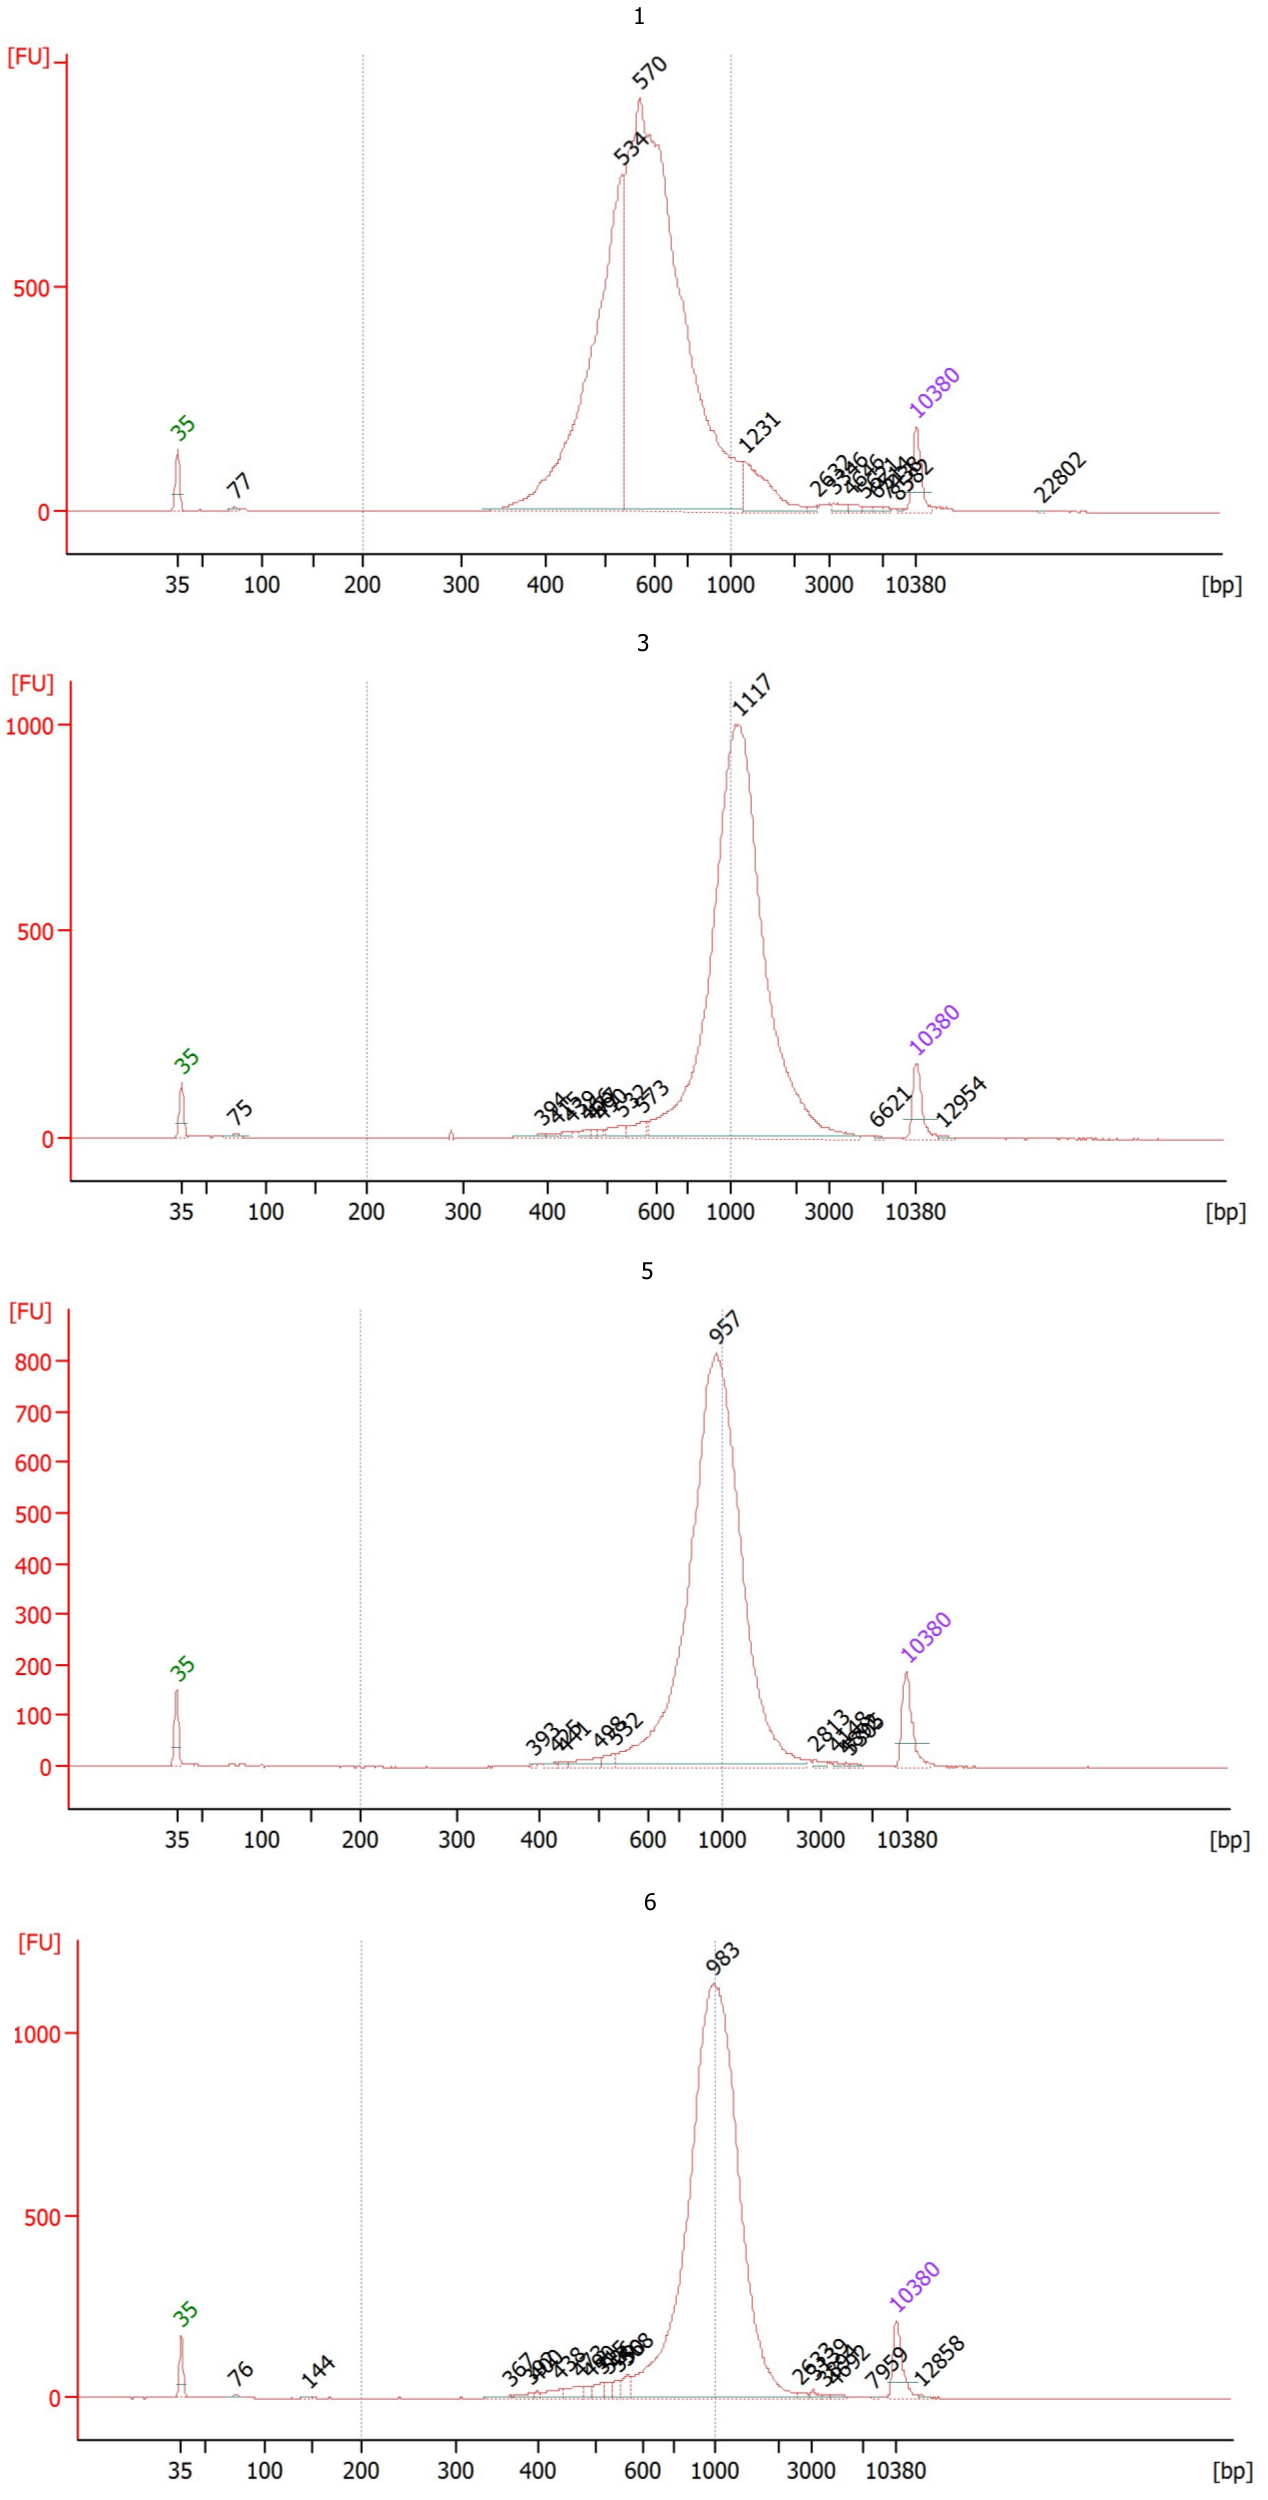
\includegraphics[width=9cm]{images/size_selection_1.png}}
\caption{Electropherograms from the high-sensitivity DNA assay of the four samples after size selection and PCR amplification.}\label{fig:sizeselection}
\end{figure}


\section{Second size selection of samples 3, 5, and 6. November 3, 2016}
I need to remove the large DNA fragments (right-side size selection). I will use the same suspesion to DNA ratio used before for right-side selection, namely 0.600:1. I have 9 $\mu$l left of each sample, which means I should use 5.4 $\mu$l of CleanPCR suspension to trap the large fragments and leave the small ones in the supernatant. Unfortunately, the supernatant will contain polyethylene glycol (PEG) and salt. Thus, I need to also apply a second load of suspension be able to elute the DNA in water. The second ratio does not need to be very tight, just to remove the very small primers that may be left over. Thus, in order to optimize the yield of small fragments, I will set it to 0.9:1. This translates in 2.7 additional $\mu$l of the CleanPCR suspension.

I performed the second size selection on samples 3, 5, and 6 without problems. I also run the amplification PCR just as the first one. I did change pipette tips. The FisherBrand tips that I was testing did not fit well the pipette, and were not accurate. The VWR tips work better with my pipettes (Nichipet EX II).


\bibliographystyle{abbrvnat}
\bibliography{notes}

\end{document}
